\documentclass{article}
\usepackage{amsmath}
\usepackage{amssymb}
\usepackage{graphicx}
\usepackage[margin=1in]{geometry}
\usepackage{hyperref}
\usepackage{caption}
\usepackage{float}
\graphicspath{{images/}}
\hypersetup{
  colorlinks=true,
  urlcolor=blue,
}
\begin{document}

\title{Game Notes}
\author{Aresh Pourkavoos}
\maketitle

Position within square stored as an odd signed integer in half-pixels,
e.g.
\begin{center}
  \begin{tabular}{|c|c|c|c|}
    \hline
    101 & 011 & 001 & 011 \\ \hline
    -3 & -1 & 1 & 3 \\ \hline
  \end{tabular}
\end{center}
Requires entities to have odd pixel dims to be centered \\
Edge/vertex states are not possible \\
Updating position requires doubling velocity first \\
Store position as $x$ and $y$ seen on screen
or relative to a square's axes? \\
Screen position: 
\begin{itemize}
\item
  Graphics and movement are easier
\item
  Collision would be most convenient by loading the current square rotated
\end{itemize}
Relative position:
\begin{itemize}
\item
  Collision is easier, just check against stored square
\item
  Need to ensure that rendering is done correctly
\end{itemize}
View splitting is decided by determinant sign:
will always give edge to cell further (counter?)clockwise \\
Vertices/edges are on the border between pixels (even position):
do not require a special case
\begin{center}
  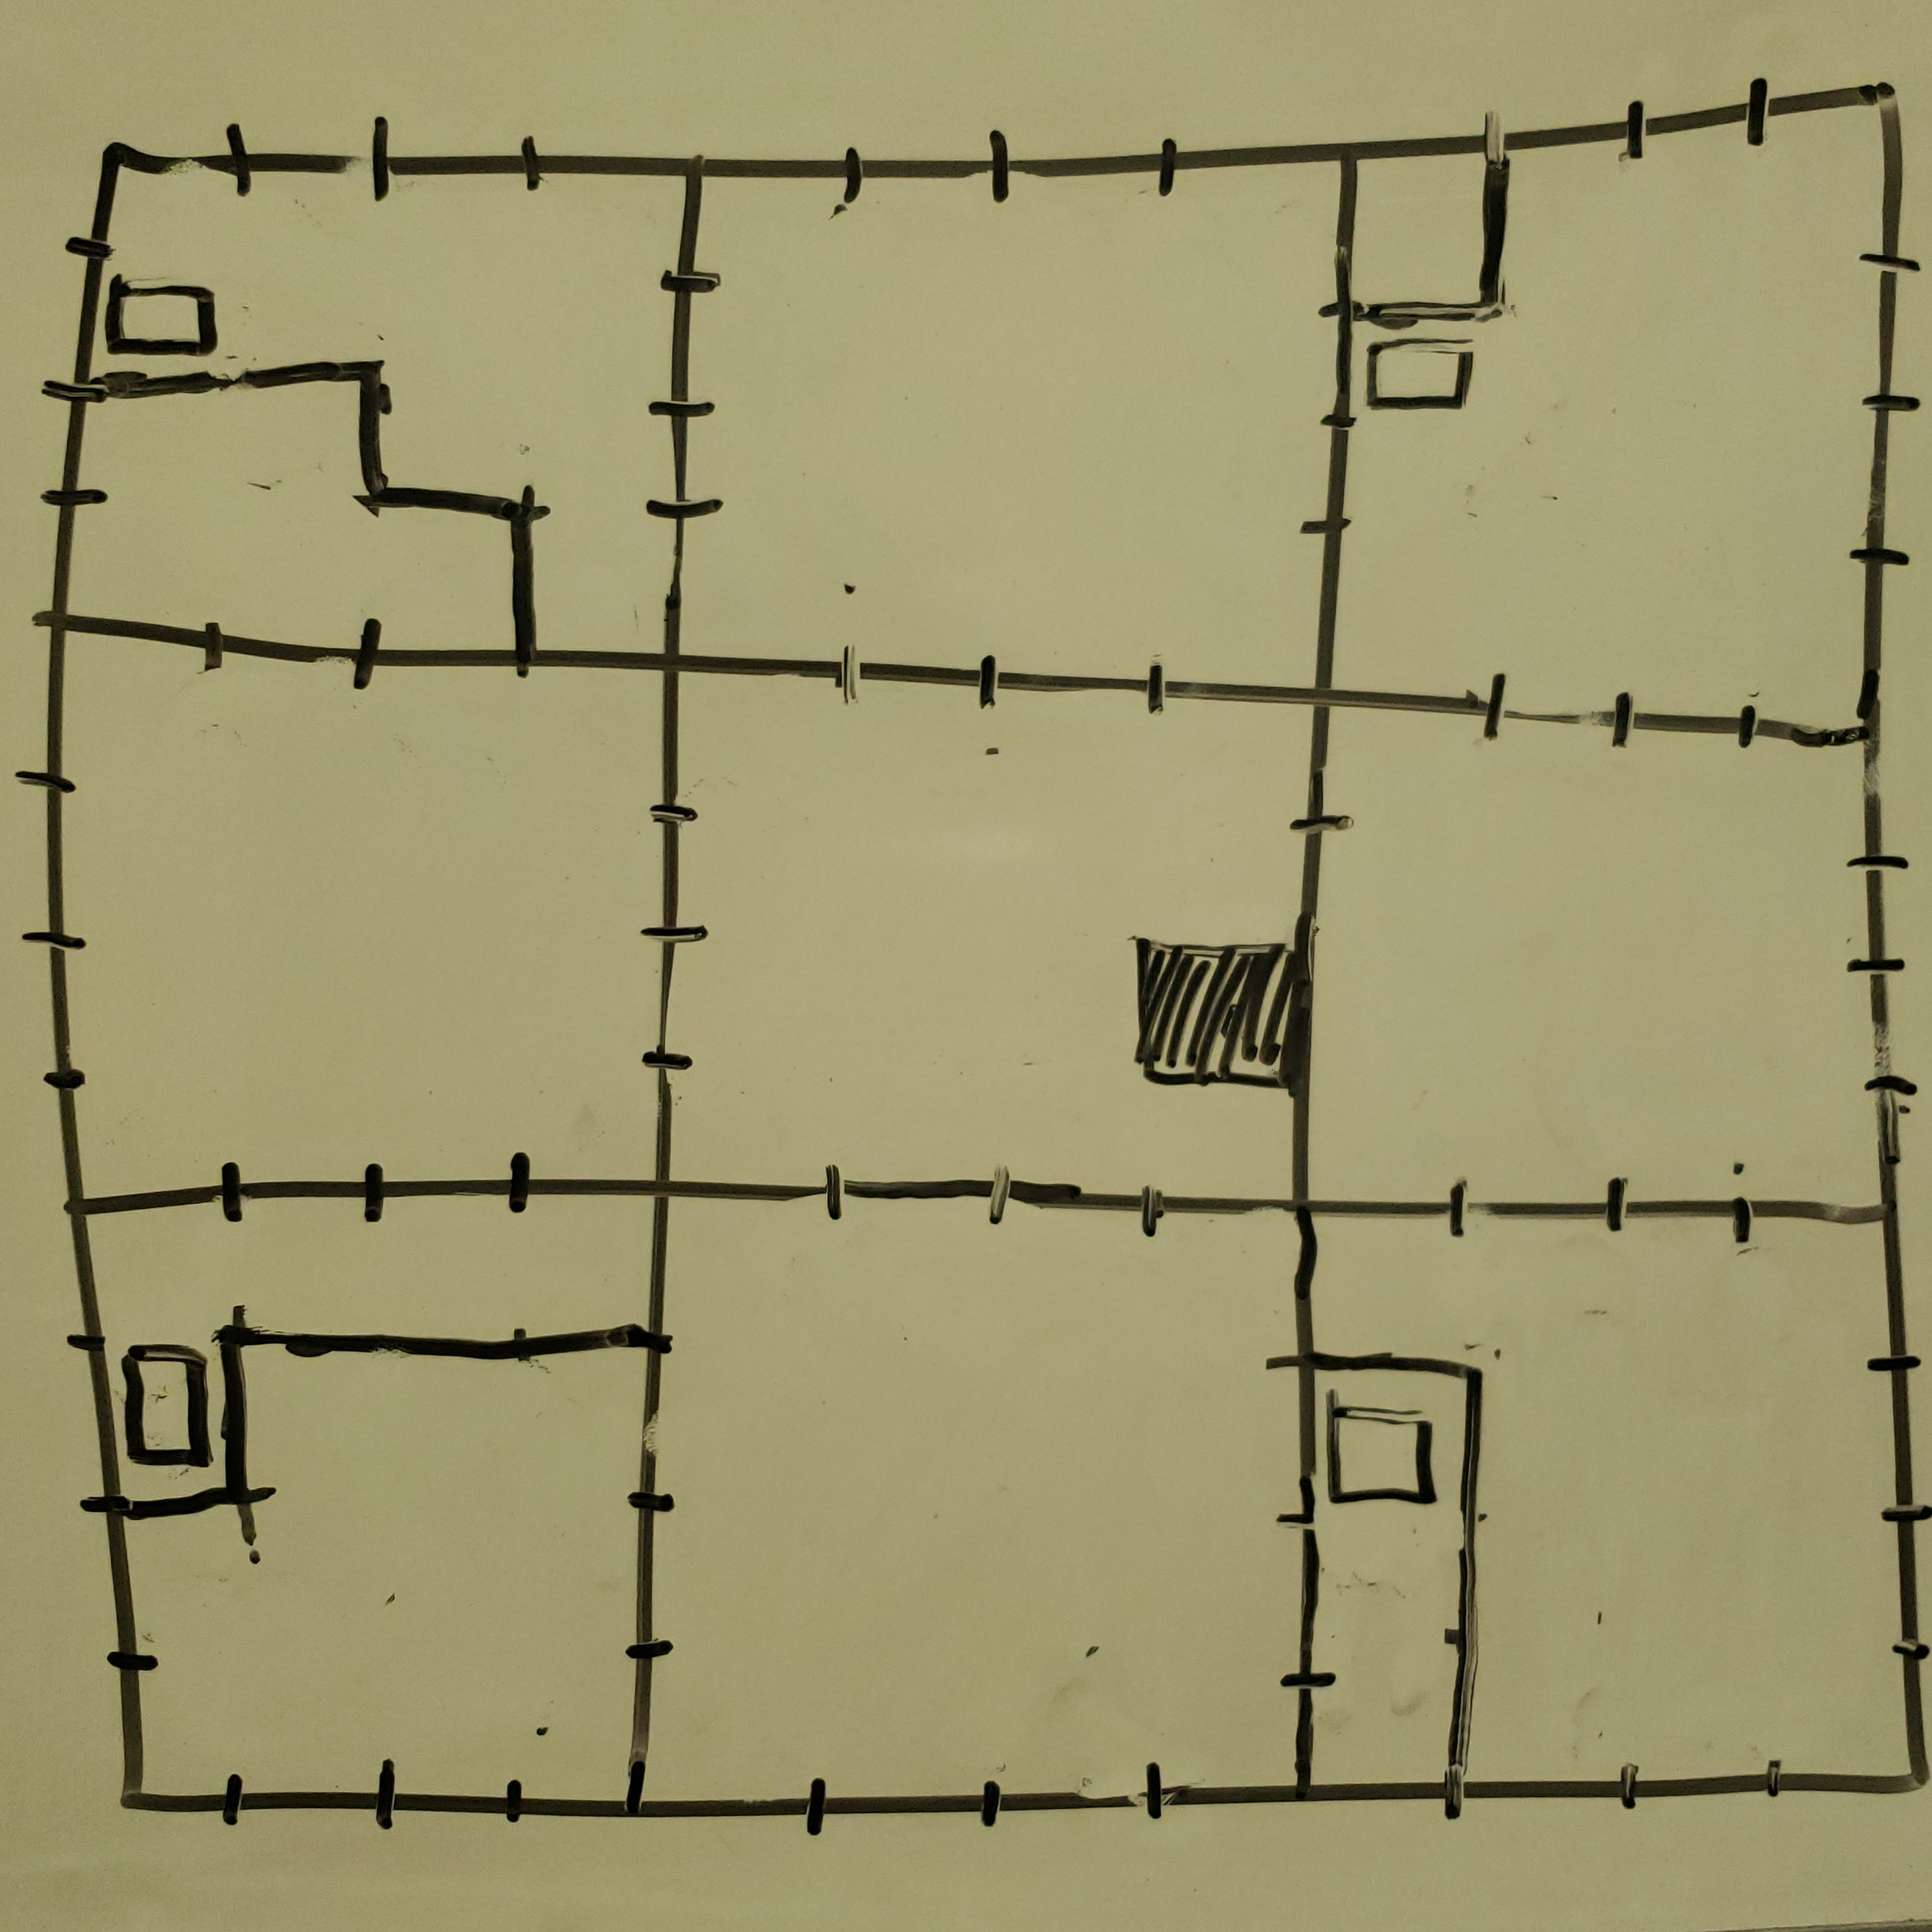
\includegraphics[width=0.5\linewidth]{grid.jpg}
\end{center}
Shaded pixel: camera \\
Lines: region boundaries \\
Inlined pixels: edge cases (given to clockwise region in this case) \\
Going through a singularity and back is a holonomy loop \\
Entity gravity is ambiguous when not in the same square as the player:
\begin{itemize}
\item
  Freeze when player leaves the square: unintuitive, esp for flat regions
\item
  Based on last player interaction: better, but initial direction must be set:
  could be none
\end{itemize}
Have ``naked'' singularities or cover them up? \\
Naked is easier to implement if accounted for
at the cost of real physics: \\
an object of finite size can't actually pass through one \\
Not checking self-collisions would obviate this
but may result in graphical glitches \\
Covering singularities would prevent glitches and restore accuracy
but might hurt level design \\
Larger squares $\rightarrow$ fewer singularities $\rightarrow$ less harm in covering them \\
Also, must be regions  accessible in only one orientation:
side longer than 2x jump height \\
However, smaller squares $\rightarrow$ more convenient to travel/execute holonomy \\
Leaning towards covering,
especially since multi- entity collisions near them can get hairy \\
Collisions near edges are inevitable,
but behavior near edges is well-defined \\
Need to distinguish between singularities and non-singular vertices:
4 squares meeting at a point \\
To resolve collisions at edges/non-singular vertices,
may need ``intermediate'' frame of reference \\
If these are necessary, may not need to bother with half-pixel positions:
allow entities centered on edge/vertex \\
But if this is the case, need to ensure that behavior is the same
regardless of if in one face or the other

%% Render method 1 (recursive): \\
%% Accept left+right boundary points, square to render,
%% position/orientation of square, quadrant \\
%% Render given square in full \\
%% Check if furthest vertex given by quadrant (``splitting vertex'') falls strictly within bounds \\
%% If not, call with same bounds/quadrant,
%% single adjacent square with new position/orientation \\
%% If so, make 2 recursive calls changing appropriate bounds to splitting vertex \\
%% Store the result of the 2nd call in a separate buffer \\
%% Could maintain a stack of buffers and add depth as an argument: depth necessary anyway \\
%% Mask buffer with line between camera and splitting vertex (anti-aliasing here!) \\
%% Overlay with original buffer \\
%% 4 base cases starting from current square with left/right bounds along x/y axes \\
%% Renders current square 4x and squares in same row/col 2x \\

%% Render method 2 (polygons): \\
%% Build a tree of regions, starting from current square \\
%% Region info: left and right boundary points, square rendered,
%% position, and orientation of square \\
%% Region is split if strictly contains singularity (i.e. not on edge) \\
%% 4 quadrants constructed separately,
%% contains duplicate regions like previous method \\
%% For each position, the regions are laid on top of each other using z depth
%% in (counter)clockwise order \\
%% Each region gets transparency based on just one separating point:
%% layer underneath gives anti-aliasing effect \\
%% Masking areas behind opaque objects should only be done at the end: \\
%% ensure consistent behavior inside/outside square containing object \\

Render method (pixel shader): \\
Build a tree of regions, starting from current square \\
Region info: left and right boundary points, square rendered,
position, and orientation of square \\
Region is split if strictly contains singularity (i.e. not on edge) \\
4 quadrants constructed separately,
contains current square 4x and squares in same row/col 2x \\
Build tree using an array/queue for BFS \\
Regions in the same position are contiguous in the queue \\
Store index of first region in array \\
Given a pixel, find position, access array for queue index,
iterate through queue until pixel is in bounds \\
Apply orientation of region to find color \\
``Raycasting'' each pixel is slower than this,
but the function will be useful later for collision resolution \\

Art style between pixel and vector:
each ``pixel'' is not a solid color but one of a few predefined shapes, \\
e.g. solid color, 2 colors split diagonally, split by circular arc \\

Physics \\
Single entity moving in static background:
all collisions are with axis-aligned surfaces \\
Collision multiplies perpendicular velocity by integer $\leq 0$,
keeps parallel velocity constant \\
Intersection point could be any rational number,
so can't store intermediate positions \\
Instead, reflect both beginning and end points across plane of collision
(adjusted for size of player), \\
recursively/iteratively resolve collision with ``mask,''
i.e. ignoring portion of trajectory ``before'' hitting wall \\
Collision state consists of beginning/end points
and rectangle to check \\
Initialized to previous frame position
and rectangle encompassing path \\
E.g. moving up+right: rectangle starts at lower left corner of starting position,
extends to top right of ending position \\
Collision with vertical surface changes only x-coordinates of beginning, end, and quadrant \\
But this can cause bugs with large players and irregular walls:
maybe rational coords are the easiest \\
45 degree slopes are possible as well,
as long as coefficient of restitution (bounciness) is odd \\
Doesn't work with pixel buffer for collisions:
need to add ``static'' entity \\

Game loop \\
Build region tree \\
Take player input \\
Update velocity accordingly (also gravity here?) \\
Resolve collisions \\
Render \\

Types of entities \\
Environmental: either stationary or on a fixed path (e.g. bouncy walls, moving platforms) \\
Collision resolution should not affect their velocities under any(?) circumstances \\
Environmental entities may intersect each other \\
Interactive: can be moved by the player (e.g. boxes) \\
Player \\
All entities are 135 degree octagons \\
8 numbers representing taxicab distance from center to sides in half-pixels \\
Ex: $3 \times 5$ rectangle has horizontal distances 3, vertical 5, diagonal 8 \\
Orthogonal distances must be odd, diagonal must be even \\
Spec: NE$\leq$N+E, 2N$\leq$NE+NW (equality implies side length 0) \\
Alternatively, could measure diagonal distance in pixels \\
Spec in this case: 2NE$\leq$N+E, N$\leq$NE+NW \\

\begin{center}
  
\includegraphics[width=0.25\linewidth]{entity.png}
\end{center}

Sides are marked as collidable or not \\
Collisions are only checked between opposing sides of entities:
makes one-way platforms possible \\
Simplest case: only need to check player vs. environment \\
Create ``virtual'' entities in adjacent faces to allow for collisions across boundaries \\

How to handle sub-pixel movement for fluidity? \\
Store sub-pixel position: more ``correct,'' but may not look good \\
Also would require additional programming for collisions
to avoid resetting sub-pixel position \\
Round sub-pixel velocity before adding: more consistent jumps between frames,
position is always an integer \\

Simple collision: 2 entities (A, B), same tile \\
%% Any opposite sides (e.g. A left, B right) pointing towards each other both before and after:
%% no collision \\
%% Is the converse true? Look at Minkowski difference
Check each pair of opposite sides (e.g. A left, B right) \\
Use adjacent sides to determine vertex locations \\
Edges of A and B trace out a parallelograms as they move \\
Need to check whether these intersect using Minkowski difference,
which is itself another parallelogram \\
Difference intersects origin $\rightarrow$ edges collide \\
Need to ensure that origin is ``passed over'' in the right direction
to allow for one-way platforms \\
Ex checking A left, B right:
A side must be non-strictly to right of B at beginning, strictly left at end \\
Find (rational) time where distance is 0: $0 \leq t < 1$ \\
Use bounciness to compute new ``starting point'' (image) and velocity \\
Ex player vs. environment: use frame of reference of environment \\

Entity passes through multiple tiles: include ``virtual'' entitites \\
Virtual entity should be created for all tiles which any part of the entity
non-strictly touches \\
How to find all of these (easily?) Assurances on entity size, etc \\
Not just all tiles, but all ``regions:'' can pass through same tile in multiple ways
e.g. Mobius strip \\

Collision resolution loop has current positions (rationals),
ending positions (integers), velocities (integers)
Only consider collisions which occur between this number (incl) and 1 (non-incl) \\
Collision location (edge) must also be (non-strictly) within bounds of tile \\
May happen on tile boundary: should not matter which one is resolved before end of loop \\

Could heavily emphasize integer-based physics: \\
discrete position in large ``cells,''
movement updates occur slowly (turn-based or on visible timer) \\
Could have interesting interplay with gravity \\
Pool-type game? \\

Ways that physics could break \\
Object crushed between two others of higher priority:
detect by overflow of denominator of time/position \\
Object sandwiched between two bouncy walls:
detect by returning perfectly(?) to previous state \\
Object bouncing between superelastic walls: also overflow(?) \\
Easy catchall fix: limit on number of iterations \\
Cleaner fix: no interactive entities (besides player),
no squeezing/crushing, speed cap \\
Player may hit multiple entities on the same edge at the same time:
use the bounciest one \\
Speed cap would also ensure that one of the following is true
about player trajectory:
\begin{itemize}
\item
  Remains within 1 tile
\item
  Crosses an edge: 2 tiles
\item
  Crosses two adjacent right-angled edges: 3 tiles
\item
  Passes through a non-singular vertex: 4 tiles
\end{itemize}



\end{document}
